\section{Motion Detector Module} \setAuthor{Richard Krammer}

    This module allows the node to detect motion in its environment. This Module can be 
    attached simultaneously with the Battery Module to the Base Module

    \subsection {Hardware - V1.1(Final)}
        The motion module has two revisions, V1.0 and V1.1. The only difference is that 
        a resisitor was removed from the V1.1 version. The schematic and layout did not 
        change. The resisitor was removed from this print and added to the Base Module
        in order to prevent the GPIO pin from floating.
    
    
        

        \subsubsection{Sensor}
            The PIR sensor EKMB1305111K is used to detect motion. This particular sensor was chosen
            for its ability to oversee a wide angel of about 150° with a range of 5m, therefor it is
            a good choice to observe corridors or rooms in a house.

            \begin{figure}[H]
                \centering
                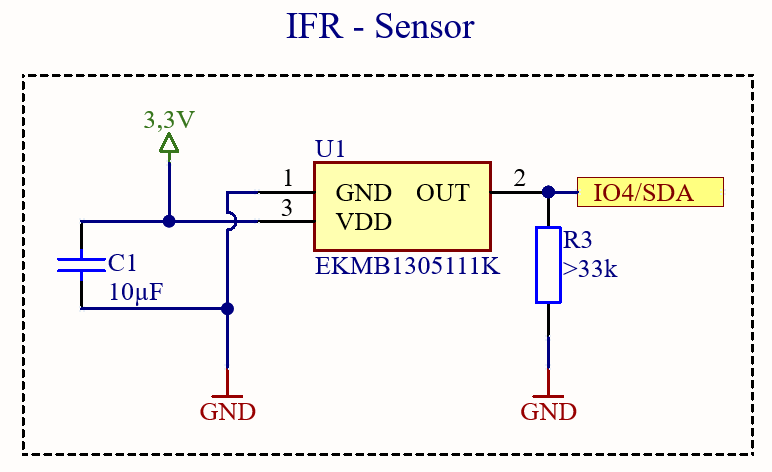
\includegraphics[width=0.4\textwidth]{assets/HW/Motion-IRF.png}
                \caption{PIR Sensor implemented in the schematic.}
            \end{figure}

        \subsubsection{Module Connector}
            The Motion Module connects with an 10-pin connector to the Base Module. It is supplied 
            with 3.3V and GND. And pin 4 is used to read the sensor.

            \begin{figure}[H]
                \centering
                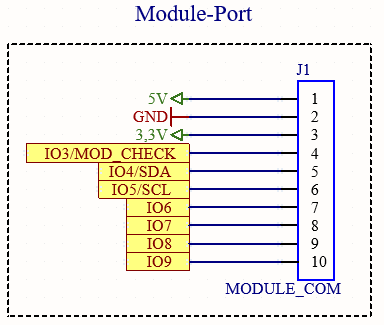
\includegraphics[width=0.4\textwidth]{assets/HW/Motion-Module-Port.png}
                \caption{Module-Connector implemented in the schematic.}
            \end{figure}

        \subsubsection{Module Detection}
            A 22kOhm resistor is connected to pin 3 to set the voltage devider.

            \begin{figure}[H]
                \centering
                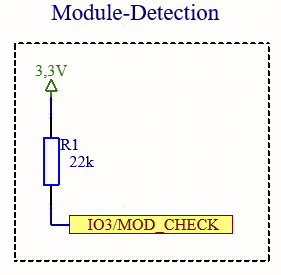
\includegraphics[width=0.4\textwidth]{assets/HW/Motion-Module-Check.png}
                \caption{Motion-Detection implemented in the schematic.}
            \end{figure}

        \subsubsection{Schematic - V1.1}
            The schematic of the Motion Module is shown in the following page.
            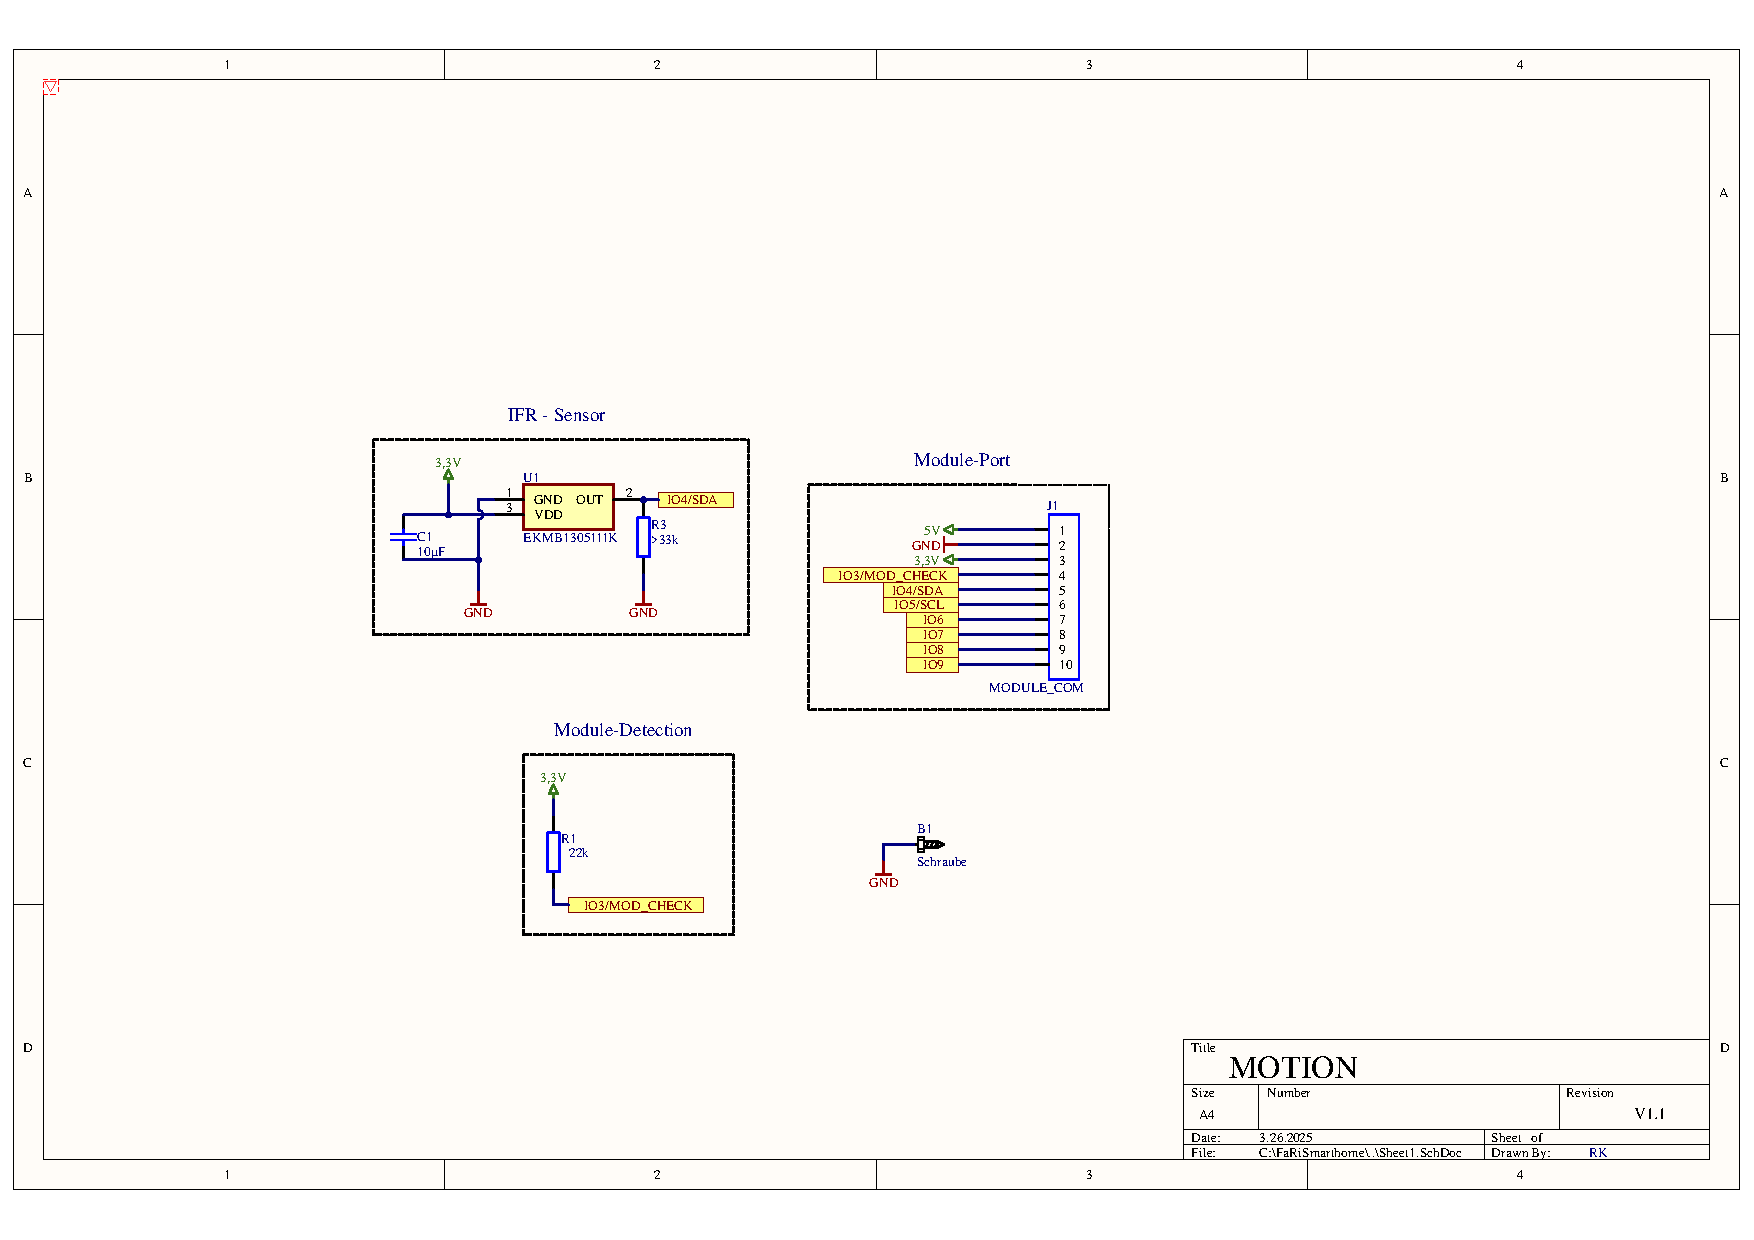
\includepdf[pages=1, angle=270, scale=1.0]{assets/HW/PDF-Schematic/Motion-V1.1.pdf}
            


        \subsubsection{PCB - V1.1}    
           
        
    \subsection {Hardware - V1.0} 
            Version 1.0 of the motion module is identical to version 1.1, except for the resistor R2.
            This resistor was removed from the motion module and added to the base module. The
            reason for this change is to prevent the GPIO pin on the base module from floating. 
            The PCB layout of the motion module is shown in the following page.